\chapter{Coordinating Distributed Systems}

\section{Two-phase commit}
	Two-phase commit is the simplest consensus protocol. It works in two phases: during phase 1 one coordinator node \textit{C} suggests a value to the other nodes and gather the responses; in phase 2, if all nodes agree, \textit{C} sends a commit command, abort otherwise.\newline
	\begin{figure}[H]
		\centering
		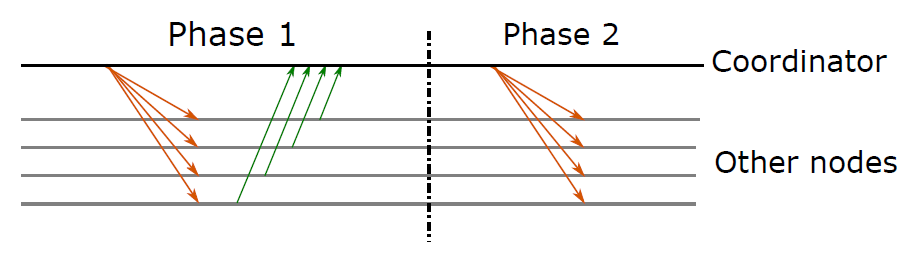
\includegraphics[width=0.8\linewidth]{images/twophasecommit.png}
	\end{figure}
	This protocol cannot make progress if there are simple failures. If \textit{C} fails in phase 1, it has to abort and retry, if it fails in phase 2, it has to replay the outcome (commit/abort). In both cases the outcome is uncertain until \textit{C} restarts.\newline
	If just one of the other nodes crashes, is slow or unreachable, the value cannot be committed.
	
\section{Paxos}
	Paxos uses state-machine replication, state machines ae fully deterministic: committed operations are executed in the same order by all state machines in the cluster.\newline
	The problem of Paxos is it is too complex and difficult to implement, there there are 5 different roles, the leader can work with a subset of the available nodes (quorum), there can be multiple proposals in the same round..
	\subsection{A simplified Paxos round}
		\subsubsection{Phase 1}
		A node in the cluster self-appoints as leader and chooses a new ballot ID. It sends a ballot proposal to the other nodes and they return the highest ballot ID they know (they can include their proposal for the value). If a majority responds with the proposed ID, the protocol can proceed.
		\begin{figure}[H]
			\centering
			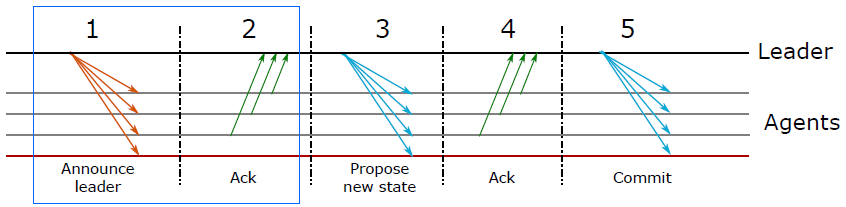
\includegraphics[width=0.8\linewidth]{images/paxos.png}
		\end{figure}
		\subsubsection{Phase 2}
		The leader resolves any conflicting proposal for the value and proposes it to the nodes. The nodes answer to the leader and, if a majority accepts the new value, it is final for this round, otherwise a new round must be started.

\section{Raft}
	\subsection{Overview}
	Raft implements distributed state machines too, it maintains a distributed log containing state machine commands.\newline
	The elected \textit{leader} handles all communications with the clients (no comms otherwise) and has the control on which entries are committed to the log.\newline
	All nodes are known in advance, the other nodes are passive replicators, periodic heartbeats are used to check if nodes are alive.\newline
	Snapshotting is used to keep the log size limited. 
	\subsection{Elections}
		At any given time each node is either a \textbf{leader}, a \textbf{follower} or a \textbf{candidate}.\newline
		Time is divided into terms, each identified by a monotonically increasing ID. All messages are labelled with a \textbf{term ID} used to identify obsolete information.\newline
		\newline
		Each node has a random timer, the \textbf{election timeout}. If anode does not receive any leader heartbeat before the timeout, it starts an election: it increments the term ID, becomes a candidate and votes for itself.\newline
		If it receives a majority of votes then it becomes a leader, if it receives a message from another leader, then it becomes a follower. No one wins before the election timeout expires again.
		\subsubsection{Election properties}
			\textbf{Safety}: there is at most one winner per term. Each voter votes only once per term and there cannot be two majorities in the same term.\newline
			\textbf{Liveness}: a leader will eventually be elected, the randomness of the timeout guarantees there will be different candidates at different times.\newline
			Faults causing new terms happen rarely compared to a second-lasting election.
	\subsection{Operation}
		Clients send commands to the current leader\newline
		The leader logs a new (uncommitted) entry\newline
		The leader sends the new entry to all nodes in the next heartbeat\newline
		Once a majority answers, the leader commits the new entry\newline
		The leader answers the client\newline
		The leader asks all nodes to commit the entry in the next heartbeat\newline
		The nodes commit the entry in their logs.
	\subsection{Failures Handling}
		\subsubsection{Leader failure}
			After the election timeout, a new leader is elected.\newline
			It will restart as a follower and set its internal term ID according to the first heartbeat message he receives. The leader will send it the missing log entries.\newline
			The client will never receive the commit ack and uncommitted entries in the followers will eventually be overwritten by the new leader.
		\subsubsection{Follower failure}
			Nothing happens and the restart process is the same as if it was leader.
		\subsubsection{50/50 vote (split majority)}
			No leader is elected, timeout expires and therefore there is a new term and a new election.\newline
			Fortunately, there is a really low probability for this to happen.
		\subsubsection{Network partition}
			The majority rule ensures only half of the partition commits new entries.\newline
			The biggest partition will elect a leader, incrementing the term ID, while the smaller one will be unable to do so (no majority).\newline
			When the partition is healed, the minority partition will receive heartbeats with a bigger term OD, uncommitted logs will be overwritten and the leader in the minority partition (if any) will immediately step down.
\section{Zoe and ZooKeeper}
	\subsection{Overview}
		When building a distributed system, one can either build his own coordination primitives (error-prone approach) or use an external coordination system, this will add external dependencies but a tested and well known system will be used.\newline
		\newline
		ZooKeeper objectives are: a simple interface, a highly available architecture and to provide common services needed by distributed systems (configuration, group management, naming, presence protocols, synchronization).
	\subsection{Architecture}
		ZooKeeper itself is distributed, for performance and fault tolerance. Clients can talk to any server but all update operation are handled by an elected leader.\newline
		Data is kept in memory for performance while snapshots and transaction logs are on persistent storage.\newline
		\newline
		ZooKeeper is AP by default: reads return local chached data\footnote{ZooKeeper writes are always synchronized through the leader.}, but the client may use the sync command to flush all caches, this will make ZooKeeper CP but there wil be a performance penalty.
		\subsubsection{ZAB}
		ZAB is the consensus protocol used by ZooKeeper (does not use state machines). It totally orders write requests using a majority of ZooKeeper processes, the leader sequences the requests and invokes ZAB atomic broadcast. Strictly ordered state updates are applied by non-leaders.\newline
		Developers focused on \textbf{strong ordering guarantees for all operations}.\newline
		\newline
		The data model is made of a hierarchical namespace (like a file system) where each node, called \textit{znode}, can contain data and have children.\newline
		Znodes can be:
		\begin{itemize}
			\item \textbf{Regular}, created and destroyed by the client
			\item \textbf{Ephemeral}, created by the client, deleted by ZooKeeper if he disconnects
			\item \textbf{Sequential}, created by the client, but the name is generated by ZooKeeper using a counter
			\item \textbf{Ephemeral + Sequential}
		\end{itemize}
		Znodes have version counters that are updated each time their content changes. A client can set a \textbf{watch} on a znode so that ZooKeeper will call him back when the data changes or a znode i created or destroyed. Watches are very useful to implement locks and leader elections with good performance.
	\subsection{Implementation}
		\subsubsection{Consensus}
		A number of processes need to agree on a value, each one proposes with \textit{create(PATH, my\_value, SEQUENTIAL)} and then each process decides:\newline
		\textit{C = getChildren(PATH)}\newline
		\textit{select znode z in C with smallest sequence suffix}\newline
		\textit{agreed\_value = getData(PATH + z)}		\subsubsection{Configuration Management}
		A number of processes need to access a common configuration which can change dynamically.\newline
		They put a watch on the configuration path and update configuration when notified of a change.
		\subsubsection{Group Membership}
		A number of processes provide the same service (load balancing), we need to leverage the ephemeral nodes.\newline
		Each process join the group so a watch is used to get notified about membership changes.